%!TEX root = ../template.tex
%%%%%%%%%%%%%%%%%%%%%%%%%%%%%%%%%%%%%%%%%%%%%%%%%%%%%%%%%%%%%%%%%%%%
%% chapter2.tex
%% NOVA thesis document file
%%
%% Chapter with the template manual
%%%%%%%%%%%%%%%%%%%%%%%%%%%%%%%%%%%%%%%%%%%%%%%%%%%%%%%%%%%%%%%%%%%%

\typeout{NT FILE chapter2.tex}%

\newcommand{\provername}[1]{\cellcolor{yellow!25}
\begin{sideways}\textbf{#1}~~\end{sideways}}
\newcommand{\explanation}[1]{\cellcolor{yellow!13}lemma \texttt{#1}}
\newcommand{\transformation}[1]{\cellcolor{yellow!13}transformation \texttt{#1}}
\newcommand{\subgoal}[2]{\cellcolor{yellow!13}subgoal #2}
\newcommand{\valid}[1]{\cellcolor{green!13}#1}
\newcommand{\unknown}[1]{\cellcolor{red!20}#1}
\newcommand{\invalid}[1]{\cellcolor{red!50}#1}
\newcommand{\timeout}[1]{\cellcolor{red!20}(#1)}
\newcommand{\outofmemory}[1]{\cellcolor{red!20}(#1)}
\newcommand{\noresult}{\multicolumn{1}{>{\columncolor[gray]{0.8}}c|}{~}}
\newcommand{\highfailure}{\cellcolor{red!50}FAILURE}

\chapter{Background}
\label{cha:background}

\glsresetall


\section{Formal Software Verification}
\label{sec:formal_software_verification}

The quest for proving that a program does what we expect it to do is so important in computer science that it became a branch of it called formal software verification. 
There are several approaches~\cite{DBLP:conf/fm/BrainP24} that try to solve this issue, each one with different characteristics, advantages and disadvantages. 
In this section, we will describe the current situation of the theoretical work and tools that constitute the background.


\subsection{Hoare Logic} 
\label{sub:hoare_logic}

Hoare logic~\cite{hoare69} is a way of reasoning about the correctness of a program, following well defined axioms and rules.
The main feature of the Hoare logic is the Hoare triple. 
The name comes from the 3 parts that constitute it: the pre-condition (\emph{P}), the program (\emph{S}) and the post-condition (\emph{Q}):
\[ \{P\} \ \textbf{S} \ \{Q\} \]

This means that if we execute \emph{S} in a state that satisfies a given pre-condition \emph{P}, then the execution finishes in a state that satisfies the post-condition \emph{Q}.
To simplify a lot, you can look at the triple as a simple logical consequence \emph{P} $\Rightarrow$ \emph{Q}.
In the same way as in the logical consequence, if \emph{P} is false, we can not say anything certain about the value of \emph{Q} (after the execution terminates, in the case of the triple).

Let us now look at an example of the usage of the Hoare triple. Consider the following program:
\[ 
\emph{S} \triangleq \textbf{if } \text{grade} \geq 10 \textbf{ then } \text{reward} := 10 \textbf{ else } \text{reward} := 0 
\]

Hoare logic can be used to prove this triple:
\[
\{ \text{grade} \geq 0 \land \text{grade} \leq 20 \} \, \textbf{S} \, \{ (\text{grade} \geq 10 \land \text{reward} = 10) \lor (\text{grade} < 10 \land \text{reward} = 0) \}
\]

This triple describes a situation where if the value of \emph{grade} is "valid" (considering grades from 0 to 20), we can say that the value of \emph{reward} will be either 0 or 10, depending if the value of \emph{grade} was less than 10 / greater or equal to 10, respectively.
It is also important to mention the difference between \emph{partial correctness} and \emph{total correctness}.
If \emph{total correctness} is what you are looking for, you need to guarantee that the execution of the program finishes.
Otherwise, you can only guarantee \emph{partial correctness}.


\subsection{Relational Hoare Logic} 
\label{sub:relational_hoare_logic}

\subsubsection{Evolution from Classical\protect\footnote{\ When we say Classical Hoare Logic, we mean the original Hoare logic developed by Tony Hoare.} Hoare Logic}
\label{sub:relational_hoare_logic_motivation}

Relational Hoare Logic~\cite{naumann2022thirtysevenyearsrelationalhoare, DBLP:conf/popl/Benton04} (RHL) is a way of reasoning about some property of two different programs or two different executions of the same program.
Some of these properties are non-interference and the equivalence of two implementations of the same algorithm, the latter being the one we are most interested in.

While classical HL reasons about the satisfaction of the post-condition if the pre-condition is satisfied, RHL analyzes the relation between two programs in terms of their corresponding evolution from a given pre-condition to a post-condition.
In other words, if programs \emph{$P_1$} and \emph{$P_2$} start in a state in which both respect the pre-condition (let us name it $\Phi$), their executions will end (if they terminate) in a state in which both respect the post-condition (let us name it $\Psi$), or none of them will.
This means that one of the programs satisfying $\Psi$ and the other not satisfying it is not valid in RHL.
That relation between the two programs is defined by the $\sim$ symbol.
This idea is known as the Hoare quadruple:
\[ \{\Phi\} \, \emph{$P_1$} \, \sim \, \emph{$P_2$} \, \{\Psi\} \]

So, why was RHL created when we already had classical HL? 
The main reason lies in the fact that the classical version does not have a direct or easy way of specifying the relation between two programs. 
This would clearly be an obstacle to this work since we aim to prove the correctness of programs by establishing a relation between them and their already proven versions or the ones that are easier to prove.
However, this thesis is definitely not the only one that relies on the connection between two different implementations of the same idea.

One common example are compiler optimizations, since they aim to make the code more performant but still outputting the same results.
Another example is represented by a "client" program that uses a abstract data type and does not care about which implementation the "server" provides.
This can happen since the implementations are expected to be observationally equivalent (i.e., to the "client" they behave the same way) and is the "server" internal logic that decides which one to choose.
That choice would depend on some characteristics that, for example, cause one implementation to be more performant than some other(s) in a given situation.


\subsubsection{Detailing RHL with examples}
\label{sub:relational_hoare_logic_examples}

Next, there are some requirements not specified previously when presenting the Hoare quadruple.
These are important details that have to be accounted for and will be described using example programs to make the explanation more tangible.
Consider the notation \emph{P$_i$.j} that will be used in this subsubsection, where \emph{i} represents a given program index, \emph{P$_i$} refers to a given program and \emph{P$_i$.j} the identifier of a variable \emph{j} in program \emph{P$_i$}.

The first example corresponds to two different programs, let us call them \emph{$P_1$} and \emph{$P_2$}, and they both contain only two assignment statements applied to the same group of variables (\emph{a, b, c}): 
\begin{tabbing}
  \hspace{2cm}\= \emph{$P_1$} \hspace{2cm} \= \emph{$P_2$} \\ 
  \> \emph{b := a + 1;} \> \emph{c := a + 2;} \\
  \> \emph{c := b + 1;} \> \emph{b := c - 1;}
  \label{tabbing:simple_equivalent_program}
\end{tabbing}

We can see that \emph{b} and \emph{c} do not change the final state of any of the programs, so, to write a Hoare quadruple that creates an equivalence between \emph{$P_1$} and \emph{$P_2$}, we need the pre-condition to assert that \emph{$P_1$.a = $P_2$.a}:
\[ \{ \Phi \} \, \emph{$P_1$} \, \sim \, \emph{$P_2$} \, \{ \Psi \} \]
\vspace{-20pt}
\[ where \ \ \Phi \triangleq \text{$P_1$.a} = \text{$P_2$.a} \]
\vspace{-25pt}
\[ and \ \ \Psi \triangleq \text{$P_1$.a} = \text{$P_2$.a} \land \text{$P_1$.b} = \text{$P_2$.b} \land \text{$P_1$.c} = \text{$P_2$.c} \]

This Hoare quadruple should be read as: \emph{For any executions of $P_1$ and $P_2$, if they guarantee the equality of their a-components, they both diverge from the post-condition or they both finish in states where their a-components, b-components and c-components have the same values
\protect\footnote{\ The values of the components of any of the programs can differ between themselves (\emph{$P_1$.a} has no relation to \emph{$P_1$.b}, for example).}.}

We now introduce the concept of separability.
If two programs \emph{$P_1$} and \emph{$P_2$} utilize disjoint sets of variables, we say that they are \emph{separable}.
In this context, this means that these two programs have their own memory, so that the variables of \emph{$P_1$} are never accessed by \emph{$P_2$} and vice-versa.
Also, in those cases we do not need to specify the program that a given variable belongs to when describing the pre and post conditions.
Below is another example to show the impact on conciseness that this creates.
Consider two programs, \emph{$P_1$}, whose variables are \{{a, b, i, j}\} and \emph{$P_2$} whose variables are \{{a', b', i', j'}\}, meaning that they are separable:
\begin{tabbing}
  \hspace{3cm}\= \emph{$P_1$} \hspace{3cm} \= \emph{$P_2$} \\ 
  \> \emph{a := 1;} \> \emph{a' := 1;} \\
  \> \emph{while a < b do} \> \emph{i' := j' * j';} \\
  \> \emph{\ \ \ \ i := j * j;} \> \emph{while a' < b' do} \\
  \> \emph{\ \ \ \ a := a * i;} \> \emph{\ \ \ \ a' := a' * i';} \\
  \> \emph{od} \> \emph{od} 
\end{tabbing}

What these programs calculate is not the focus here but notice a subtle, yet relevant difference: \emph{i' := j' * j';} is out of the loop in \emph{$P_2$}.
This is a common compiler optimization called \emph{invariant hoisting}.
\emph{Why would you waste time performing a task several times if you can do it only once and get the same output?}
In this example, the Hoare quadruple would be:
\[ \{ \Phi \} \, \emph{$P_1$} \, \emph{\textasciitilde} \, \emph{$P_2$} \, \{ \Psi \} \]
\vspace{-20pt} 
\[ \text{where} \ \ \Phi \triangleq (b = b') \land (j = j') \]
\vspace{-25pt} 
\[ \text{and} \ \ \Psi \triangleq (a = a') \land (b = b') \land (i = i') \land (j = j') \]

Since the previous values in \emph{a} and \emph{i} (respectively \emph{a'} and \emph{i'}) are discarded by the assignments made to these variables, they will have no effect on the final state, so they do not appear in the pre-condition.
On the other hand, to make sure that the components of \emph{$P_1$} and \emph{$P_2$} hold the same values after the executions terminate, we must assert that the b-components and j-components are equal in the initial state of the programs. 

Furthermore, there is a special case of the usage of the Hoare quadruple that does not challenge any concept described before.
Usually, in the context of the Hoare quadruple, we consider that the programs \emph{$P_1$} and \emph{$P_2$} are different, but what would happen if they are exactly the same?
Well, since they are equal letter for letter, it is natural that they will always output the same results given the same inputs.

Finally, consider again two equal programs \emph{$P_1$} and \emph{$P_2$}.
The way one should look at the transformation of Hoare triples into Hoare quadruples is that if \{$\Phi$\} \emph{$P_1$} \emph{\textasciitilde} \emph{$P_2$} \{$\Psi$\} is true, then \{$\phi$\} \emph{$P_1$} \{$\psi$\} will be true as well.


\subsubsection{Axioms and Inference Rules}
\label{sub:relational_hoare_logic_formal_proof_rules}

Consider the following grammar, that will be used in the rules in this subsubsection.
Let \emph{n} represent any integer number \{... -1, 0, 1 ...\}, \emph{x} any integer variable of a given program and \emph{a} any array variable.
Let \emph{e} be the set of integer expressions, \emph{b} the set of boolean expressions and \emph{c} the set of program expressions (also called commands or statements).
The syntaxes of \emph{e}, \emph{b} and \emph{c} are given by the following extended BNF definition:\\ \\
\noindent\hspace*{1em}
\begin{minipage}{\dimexpr\linewidth-2em\relax}
\[\begin{aligned} 
& E ::= \, n \,|\, x \,|\, E_1 + E_2 \,|\, E_1 - E_2 \,|\, E_1 * E_2 \,|\, E_1 / E_2 \,|\, ... &\\
& B ::= \, \textbf{true} \,|\, \textbf{false} \,|\, \neg B \,|\, B_1 \lor B_2 \,|\, B_1 \land B_2 \,|\, B_1 = B_2 \,|\, B_1 < B_2 \,|\, ... &\\
& C ::= \, \textbf{skip} \,|\, \textbf{assert} (B) \,|\, x := E \,|\, a[E_1] := E_2 \,|\, C_1;C_2 \,|\, \textbf{if}\, B\, \textbf{then}\, C_1\, \textbf{else}\, C_2 \,|\, \textbf{while}\, B\, \textbf{do}\, C \,|\, ... &
\end{aligned}\]
\end{minipage}\\ \\

The ellipses above mean that other forms of integer expressions could be added according need.
It is also important to note that this language does not consider indentation, so we will use that advantage to make reading easier below.
Finally, assume, for the rules in this subsubsection, that the two given programs \emph{$C_1$} and \emph{$C_2$} are separable.

To derive valid Hoare quadruples, there are axioms and inference rules that reason about the relation between two programs~\cite{DBLP:journals/jlp/BartheCK16}.
We can divide these rules in at least three sets that increment the former set with some additional rules, meaning that there is the simplest set, the base set and the extended set.
The simplest set has limitations that we will discuss after presenting them, but is the best starting point:

\begin{figure}[h]
  \centering
  \begin{mathpar}
  \inferrule*[right=skip]
  { }
  {\vdash \{ \Phi \} \ \textbf{skip} \sim \textbf{skip} \ \{ \Phi \}}
  
  \inferrule*[right=assignment]
  { }
  {\vdash \{ \Psi[x_1 \mapsto E_1][x_2 \mapsto E_2] \}  \ x_1 := E_1 \sim x_2 := E_2 \ \{ \Psi \}}
  
  \inferrule*[right=sequencing]
  {\vdash \{ \Phi \} \ C_1 \sim C_2 \ \{ \Theta \} \\\vdash \{ \Theta \} \ C'_1 \sim C'_2 \ \{ \Psi \}}
  {\vdash \{ \Phi \} \ C_1; C'_1 \sim C_2; C'_2 \ \{ \Psi \}}
  
  \inferrule*[right=conditional]
  {\shortstack{%
    $\vDash \Phi \rightarrow (B_1 = B_2)$ \\[0.5ex]%
    $\vdash \{ \Phi \land B_1 \} \ C_1 \sim C_2 \ \{ \Psi \}$ \\%
    $\vdash \{ \Phi \land \neg B_1 \} \ C'_1 \sim C'_2 \ \{ \Psi \}$%
  }}
  {\vdash \{ \Phi \} \ \textbf{if } B_1 \textbf{ then } C_1 \textbf{ else } C'_1 \ \textbf{fi} 
  \sim \textbf{if } B_2 \textbf{ then } C_2 \textbf{ else } C'_2 \ \textbf{fi} \ \{ \Psi \}}

  \inferrule*[right=while]
  {\vdash \{ \Phi \land B_1 \} \ C_1 \sim C_2 \ \{ \Phi \} \\\vDash \Phi \rightarrow (B_1 = B_2)}
  {\vdash \{ \Phi \} \ \textbf{while } B_1 \ \textbf{do } C_1 \ \textbf{od} \sim 
  \textbf{while } B_2 \ \textbf{do } C_2 \ \textbf{od} \ \{ \Phi \}}
  
  \inferrule*[right=weakening]
  {\vDash \Phi' \rightarrow \Phi \\\vdash \{ \Phi \} \ C_1 \sim C_2 \ \{ \Psi \} \\\vDash \Psi \rightarrow \Psi'}
  {\vdash \{ \Phi' \} \ C_1 \sim C_2 \ \{ \Psi' \}}

  \end{mathpar}
  \caption{Simplest set of rules of RHL.}
\end{figure}
  
This set of rules has some considerable limitations however: both programs \emph{$C_1$} and \emph{$C_2$} must have the same shape and execute in lockstep.
This creates a situation where we can not derive a simple Hoare quadruple like \{$\Phi$\} \emph{C}; \textbf{skip} \emph{\textasciitilde} \emph{C} \{$\Psi$\}.
To allow this and other important derivations, we present next other 4 rules that enable the separate reasoning of \emph{$C_1$} and \emph{$C_2$}.
Together with the rules of the simplest set, these rules constitute the base set:

\begin{figure}[h]
  \centering
  \begin{mathpar}

  \inferrule*[right=assignment-L]
    {\vdash \{ \Phi[x \mapsto E] \} \; \textbf{skip} \sim C \; \{ \Psi \}}
    {\vdash \{ \Phi \} \; x := E \sim C \; \{ \Psi \}}

  \inferrule*[right=assignment-R]
    {\vdash \{ \Phi[x \mapsto E] \} \; C \sim \textbf{skip} \; \{ \Psi \}}
    {\vdash \{ \Phi \} \; C \sim x := E \; \{ \Psi \}}

  \inferrule*[right=conditional-L]
    {\vdash \{ \Phi \land B \} \; C_1 \sim C \; \{ \Psi \} \\ 
    \vdash \{ \Phi \land \neg B \} \; C_2 \sim C \; \{ \Psi \}}
    {\vdash \{ \Phi \} \; \textbf{if} \; B \; \textbf{then} \; C_1 \; \textbf{else} \; C_2 \; \textbf{fi} \sim C \; \{ \Psi \}}

  \inferrule*[right=conditional-R]
    {\vdash \{ \Phi \land B \} \; C \sim C_1 \; \{ \Psi \} \\ 
    \vdash \{ \Phi \land \neg B \} \; C \sim C_2 \; \{ \Psi \}}
    {\vdash \{ \Phi \} \; C \sim \textbf{if} \; B \; \textbf{then} \; C_1 \; \textbf{else} \; C_2 \; \textbf{fi} \; \{ \Psi \}}
    
  \end{mathpar}
  \caption{Base set of rules of RHL.}
\end{figure}

The base set of rules of RHL is incomplete, since it does not provide a way to reason about programs whose loop structures differ or, even when they do not, the pre-condition is not strong enough to prove that the loops execute in lockstep.
This problem can be overcome when we the extend the base set with one more rule: self-composition.


\begin{figure}[h]
  \centering
  \begin{mathpar}

  \inferrule*[right=self-composition]
    {\vdash \{ \Phi \} \; C_1 ; C_2 \; \{ \Psi \}}
    {\vdash \{ \Phi \} \; C_1 \sim C_2 \; \{ \Psi \}}
    
  \end{mathpar}
  \caption{Extended set of rules of RHL.}
  \label{fig:extended_rules_rhl}
\end{figure}

Note that the premise of this rule is not a Hoare quadruple but a Hoare triple since there is no \emph{\textasciitilde} operator, only a sequence of \emph{$C_1$} and \emph{$C_2$} within a single program.
This triple can also be presented as the following quadruple:
\vspace{-4pt} 
\[ \{\Phi \land \Phi'\} \, \emph{$C_1 ; C_2$} \, \sim \, \emph{$C_1' ; C_2'$} \, \{ \Psi \land \Psi' \} \]
\vspace{-18pt} 

If we keep the programs \emph{$C_1;C_2$} and \emph{$C_1';C_2'$} \emph{separable} by renaming their variables and if \emph{$\Phi$ = $\Phi$'} and \emph{$\Psi$ = $\Psi$'}, we get to the self-composition rule presented before.
Another way of looking at self-composition is that it reduces a Hoare quadruple into a Hoare triple by transforming the two related programs \emph{$C_1$} and \emph{$C_2$} into a new one that executes them in sequence (\emph{$C_1; C_2$}).
Finally, it is important to mention that relative completeness of the simplest or base sets of rules of RHL extended with self-composition follows immediately from relative completeness of self-composition ~\cite{DBLP:journals/jlp/BartheCK16}.


\section{OCaml}
\label{sec:ocaml}

\subsection{History \& Characteristics} 
\label{sub:overview}

OCaml~\cite{ocaml} is a general purpose programming language that was released in 1996 at the National Institute for Research in Digital Science and Technology (Inria).
It is usually seen as an extension of Caml (a dialect of the Meta Language) that includes object-oriented features, making OCaml a very versatile language.
Besides supporting the functional, imperative and object-oriented approaches, it is also a language that can be either interpreted or compiled, to either bytecode or native code.
Regarding its type system, OCaml comes with a strong and static type system that also features type inference.

Although the imperative programming paradigm is still more popular than its functional counterpart, the latter has been conquering space inside the universe of programming languages whose focus is on the imperative/object-oriented approach; for example, Java and Kotlin.
Java received its first functional features in version 1.8~\cite{java}, released in 2014 and they have been expanding since.
Kotlin, firstly released in 2016, was already designed with the functional style in mind~\cite{kotlin}.


\subsection{Relevance} 
\label{sub:relevance}

The relevance of OCaml and functional programming languages in general is an important question that I have asked myself several times in the past, and not only because the first contact with this paradigm was challenging.
Although I do not question the relevance of these languages anymore because of the evidence that I will show next, I still think that it is not an unexpected concern amongst computer science students.
I am mentioning this because the majority of jobs and businesses in the field require people for front-end development (with Javascript), back-end development (mostly with imperative languages) or, more recently, AI-related work (mostly with Python or other science-oriented languages).
There is, although, strong evidence that OCaml is far from being an "academia only" programming language.
OCaml is used in tech giants such as Meta and Microsoft, in Bloomberg L.P. (that even created an OCaml to Javascript compiler backend), in popular tools like Docker and in many other companies~\cite{ocaml_companies}.
But there is more.

Here are a few impressive examples of what this programming language has been used to build: 
\begin{enumerate}
  \item Alt-Ergo~\cite{altergo}, a popular SMT solver that has presence in Cameleer;
  \item Coq~\cite{coq}, a formal proof management system;
  \item and even the web version of Facebook Messenger~\cite{messenger}!
\end{enumerate}

\subsection{Code Examples} 
\label{sub:examples_ocaml}

In this subsection, we will look at a simple Ocaml code example that determines the greatest common divisor of two given numbers, \emph{a} and \emph{b}.
The first implementation represents the use of the functional paradigm while the second demonstrates how to use imperative constructs in this language.

\begin{ocamlsmall}
  let rec gcd (a: int) (b:int) : int =
      if b = 0 then a
      else gcd b (mod a b) 
\end{ocamlsmall}

\begin{ocamlsmall}
  let gcd_iter (a0: int) (b0: int) : int =
      let b = ref b0 in
      let a = ref a0 in
      while !b <> 0 do
          let tmp = !a in
          a := !b;
          b := tmp mod !b
      done;
      !a
\end{ocamlsmall}

Next there are some notes about the syntax and semantics in the context of these examples. 
Since OCaml supports the functional and imperative paradigms, it distinguishes between immutable variables (actually not present in the programs shown) and memory references, therefore the different syntax for the binding of each one: 
\[ \emph{let x = 3 (variable)} \]
\vspace{-25pt}
\[ \emph{let y = ref 4 (reference)} \]

The \emph{rec} keyword tells the compiler/interpreter that it is fine if the function calls itself, reducing the risk of the programmer using recursion by accident.
OCaml is also sharp enough to understand these programs correctly even if we did not specify the types of the function or its arguments.
Finally, the \emph{let} keyword can be used to define a function or create a binding, something rather uncommon for someone with an imperative background.


\section{Why3}
\label{sec:why3}

Why3 is a platform whose objective is the verification of programs in a deductive way, presenting it self as a \emph{"a front-end to third-party theorem provers"}~\cite{why3}.
These several theorem provers can be put to work together and vary greatly in nature, ranging from SMT solvers (for example, Z3 or cvc5) to TPTP provers and even interactive proof assistants (such as Coq or Isabelle).
Under the hood, Why3 is an OCaml library, implemented in the form of an API.
It features a CLI, a GUI and a benchmark tool to compare the performance of the different provers available.

When we want to verify the correctness of a given program, we need to ensure that the input code is written in WhyML~\cite{DBLP:conf/esop/FilliatreP13}, since that is the language that Why3 expects.
WhyML can be considered a ML dialect and is simultaneously a specification and a programming language that serves as an intermediary language between C, Java or Ada programs and the verification conditions (VCs) generated by Why3.

The most used WhyML specification keywords are precisely the ones present in the example in the next \hyperref[subsec:why3_example]{subsection}, \emph{requires} and \emph{ensures}.
These represent the pre-conditions and post-conditions, respectively.
Besides those, the \emph{variant} and \emph{invariant} keywords are also very common.
Loops in this language are annotated with invariants, through the use of the \emph{invariant} keyword.
While loops specifically and recursive functions benefit greatly from the \emph{variant} keyword, which represents a way of showing that the program does not run forever.

\subsection{Example}
\label{subsec:why3_example}

As a way of demonstrating how Why3 works in practice, here is a preview of what is possible to do with product programs, an important concept which we will discuss in detail in the next chapter.
If we want to prove that the original and the transformed programs are equivalent, we can write a third program that combines the first two, a \emph{product program}.

The original program is based on only two assignment instructions: \emph{y := x + 1;} and \emph{z := y + 1;}.
To make the programs separable, we renamed \emph{x}, \emph{y} and \emph{z} in the original program to \emph{x1}, \emph{y1} and \emph{z1} and in the transformed program to \emph{x2}, \emph{y2} and \emph{z2}.
The product program establishes that, if the values of the variables \emph{x1} and \emph{x2} are the same before the function \emph{product} starts, it is guaranteed that \emph{y1 = y2} and \emph{z1 = z2}.
And, since there is no assignment to any of the x-components, \emph{x1 = x2} will also be true if the pre-condition is respected.

There was no need for human intervention in verifying the product program, as the SMT solver Z3 completed the proof in under a second.

\begin{figure}
  \centering
  \begin{subfigure}[b]{0.45\textwidth}
    \begin{minipage}[t]{\linewidth}
      \textbf{Original program}
      \begin{whylang}
        use int.Int
      
        val ref x : int
        val ref y : int
        val ref z : int
      
        let original ()
          =
          y <- x + 1; 
          z <- y + 1;
      \end{whylang}
    \end{minipage}
  \end{subfigure}
  \hfill
  \begin{subfigure}[b]{0.45\textwidth}
    \begin{minipage}[t]{\linewidth}
      \textbf{Transformed program}
      \begin{whylang}
        use int.Int
      
        val ref x : int
        val ref y : int
        val ref z : int
      
        let transformed ()
          =
          z <- x + 2; 
          y <- z - 1;
      \end{whylang}
    \end{minipage}
  \end{subfigure}
  \hfill
  \begin{subfigure}[b]{0.9\textwidth}
    \begin{minipage}[t]{\linewidth}
      \textbf{Product program}
      \begin{whylang}
        use int.Int
      
        val ref x1 : int
        val ref x2 : int
        val ref y1 : int
        val ref y2 : int
        val ref z1 : int
        val ref z2 : int
      
        let product ()
          requires { x1 = x2 }
          ensures { y1 = y2 }
          ensures { z1 = z2 }
          =
          y1 <- x1 + 1; 
          z2 <- x2 + 2;
          z1 <- y1 + 1;
          y2 <- z2 - 1;
      \end{whylang}
    \end{minipage}
  \end{subfigure}
  \caption{Program based on assignments.}
  \label{fig:why3_example}
\end{figure}

\begin{table}[!h]
  \begin{center}
  \begin{tabular}{|l|l|l|l|c|}
    \hline \multicolumn{2}{|c|}{Proof obligations } & \provername{Z3 4.13.0} \\ 
    \hline
    \explanation{VC for product}  & \explanation{postcondition} & \valid{0.01} \\ 
    \cline{2-3}
    & \explanation{postcondition} & \valid{0.00} \\ 
    \hline 
  \end{tabular}
  \caption{Program based on assignments verification results.}
  \end{center}
\end{table} 


\FloatBarrier
\section{GOSPEL}
\label{sec:gospel}

GOSPEL~\cite{DBLP:conf/fm/ChargueraudFLP19} (Generic Ocaml SPEcification Language) is a tool-agnostic specification language for OCaml that allows one to verify the correctness of a program (there are other purposes but this is the most interesting for this work).
GOSPEL is based in Separation Logic and significantly improves the experience of the people that write or read the specifications, by making them much more concise.
Let us reconsider the code presented in this \hyperref[sub:examples_ocaml]{subsection}, but this time also show the GOSPEL specification for that program:

\begin{gospel}
  (*@ function rec gcd (a: int) (b:int) : int =
      if b = 0 then a
      else gcd b (mod a b) *)
  (*@ requires a >= 0
      requires b >= 0
      variant b *)
\end{gospel}

\begin{gospel}
  let gcd_iter (a0: int) (b0: int) : int =
    let b = ref b0 in
    let a = ref a0 in
    while !b <> 0 do
        (*@ invariant 0 <= !b
            invariant 0 <= !a
            invariant gcd a0 b0 = gcd !a !b
            variant !b *)
        let tmp = !a in
        a := !b;
        b := tmp mod !b
    done;
    !a
  (*@ result = gcd_iter a0 b0
      requires a0 >= 0
      requires b0 >= 0
      ensures result = gcd a0 b0*)
\end{gospel}

Although this is a simple program, we can already notice what a typical GOSPEL specification looks like.
If we are dealing with a functional piece of code usually there will be a few \emph{requires} clauses (could be none as well) at the beginning of the specification, representing the pre-conditions.
After that, since these implementations use recursion most of the time, there will be one or more \emph{variant} clauses, indicating what variables vary each time the function is called.
This serves as a guarantee that the recursion does not go forever.
In this implementation, \emph{variant b} is enough but we could eventually reason about how \emph{a} varies over the execution of the program. 
Regarding the pre-conditions, this particular example states that \emph{a} and \emph{b} need to be non negative integer numbers, since the greatest common divisor of any two negative numbers will always be 0.
Finally, we have a single post-condition \emph{ensures result = gcd a0 b0} that guarantees that for any input, the two different implementations will output the same result. 


\section{Cameleer}
\label{sec:cameleer}

Cameleer is a tool that aids automated deductive verification of OCaml programs.
It relies on GOSPEL for the specification of the code and on Why3 to effectively verify the program.
The limitations of the powerful Why3 tool and the reason for the creation of Cameleer start here: Why3 does not accept code that is not written in its intermediary language: WhyML.
Now imagine wanting to verify your codebase with years and years of contributions, with maybe more than a million lines of code.
Why3 would force you to translate OCaml into WhyML, \emph{all by hand}. 
And only after that you would write the specification.
Two obvious things come to mind: no one wants to do that job and if someone had to do it, they would very quickly start wondering if there is a tool that could help them, or even better, do that repetitive work instead of them.
So, how is Cameleer able to save those poor programmers?

\begin{figure}[htbp]
  \centering
  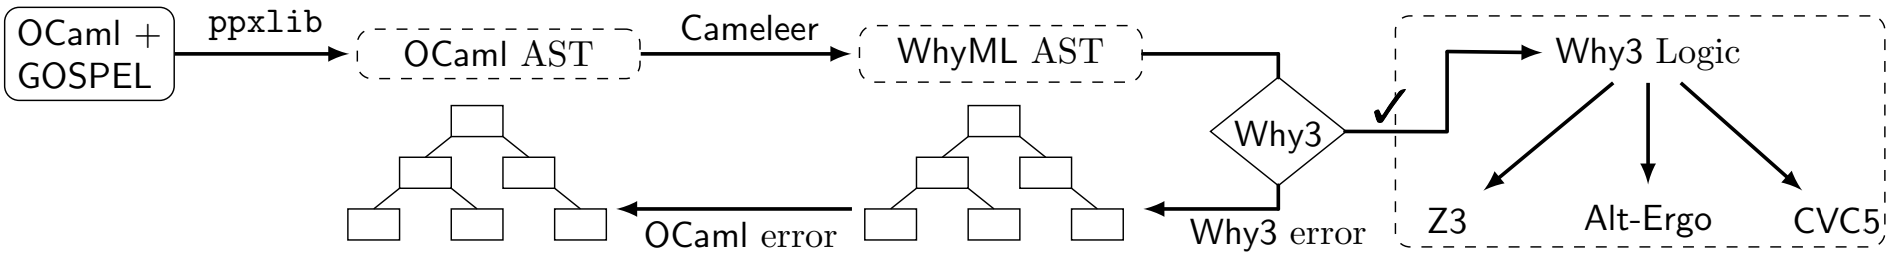
\includegraphics[max width=\textwidth]{cameleer_pipeline}
  \caption{Architecture and verification pipeline, taken from ~\cite{DBLP:conf/cav/PereiraR20}.}
  \label{fig:cameleer_pipeline}
\end{figure}

The Cameleer pipeline is constituted by 4 different steps, the last one being different depending on whether Why3 detects errors in the translated code or not.
The first step is to parse and change the abstract syntax tree of the input OCaml program (that contains GOSPEL annotations), using \emph{ppxlib}, a library that is part of the GOSPEL ecosystem\protect\footnote{\ https://github.com/ocaml-gospel/gospel}.
In the second step, the GOSPEL annotations are processed by a special parser/type-checker that converts the specification into nodes that become part of the previous OCaml AST.
The third step consists in Cameleer itself translating the complete AST into a description in WhyML that is equivalent; Why3 then takes that as input.
In step four, if the Why3 type-and-effect system is not able to validate the input generated in the previous step, the problems are shown in the context of the input OCaml code, the one that is submitted by the user. 
Alternatively, if no errors are found, a series of verification conditions are the output of the respective VCGEN.
Those VCs should then be unraveled by the solvers featured in Cameleer or, if they are not able to do all the work automatically, this tool also allows human intervention to discharge more complex statements.

\subsection{Example}
\label{subsec:cameleer_example}

We will now demonstrate the execution of the verification of a GOSPEL annotated OCaml program, using the code presented in the previous \hyperref[sec:gospel]{section}.
To start the verification, assuming the code is saved in a file called \textbf{gcd.ml}, we use the following command: \textbf{cameleer gcd.ml}.
This will feed our code to the Cameleer pipeline and, even if there are errors, a new window with the Why3 GUI will appear.

Now, we can use the \textit{Split VC} strategy (\underline{Tools} -> \underline{Strategies} -> \underline{Split VC}) to separate our bigger goal into several, smaller and simpler VCs, for each implementation.
In this case, if we use the \textit{Auto level 0} strategy (\underline{Tools} -> \underline{Strategies} -> \underline{Auto level 0}) on the \textbf{gcd.ml} goal, our proof successfully terminates.

\begin{figure}[htbp]
  \centering
  \begin{adjustbox}{frame,max width=\textwidth}
    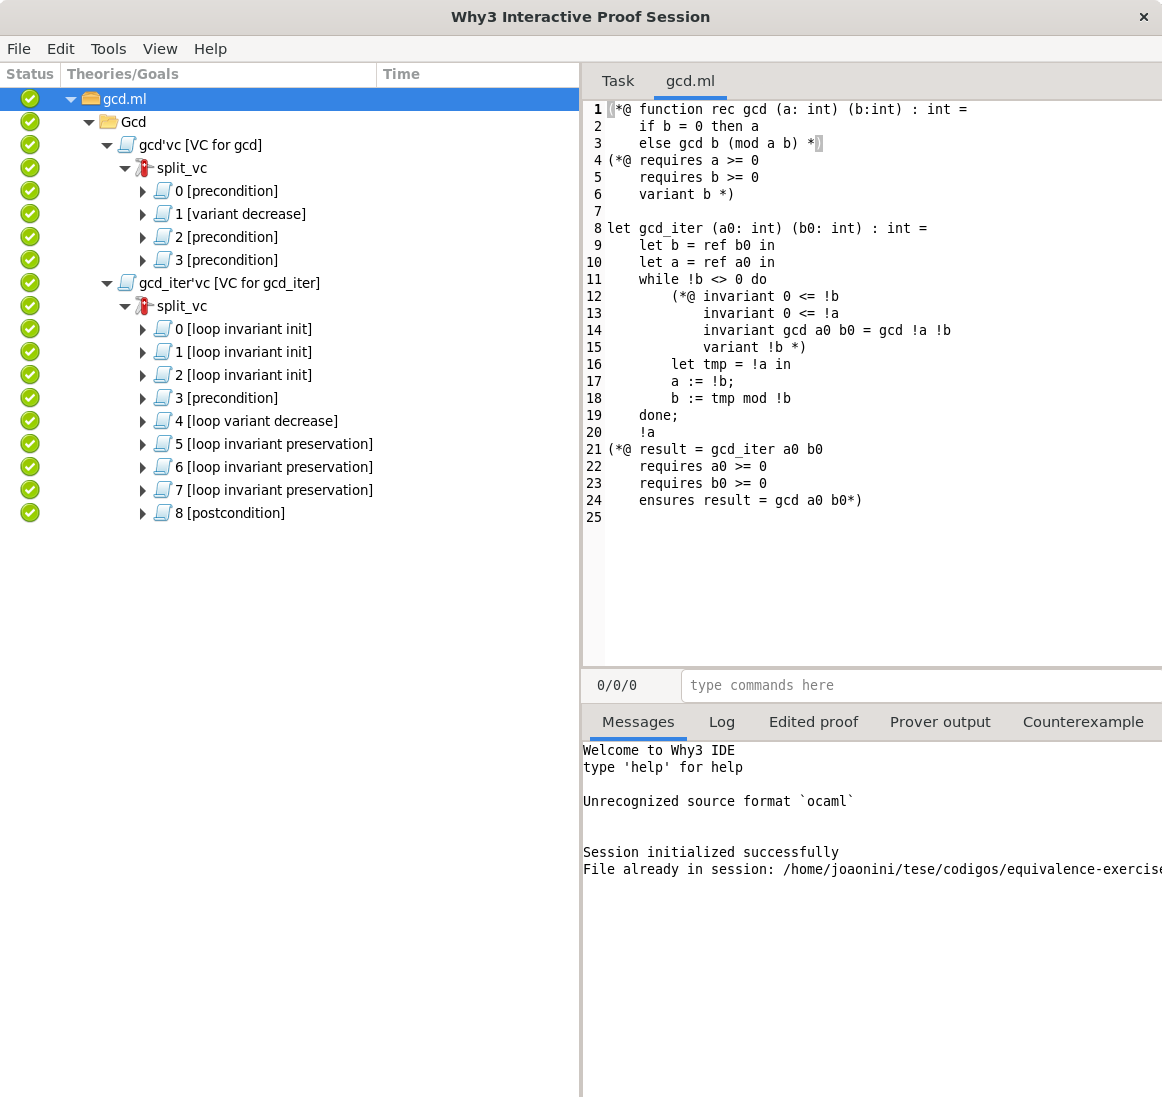
\includegraphics{gcd_why3}
  \end{adjustbox}
  \caption{Verifying \textbf{gcd.ml} with the Why3 IDE.}
  \label{fig:gcd_why3}
\end{figure}

You can now get automatically generated Latex code that shows how much time each VC took to be proven, using the command \textit{why3 session latex -o proof\textunderscore tex test}.
Do not forget to create the proof\textunderscore tex directory, otherwise you will get an error.
The Latex code for this example will look like the following.
As you can see, CVC5 was the prover used and it took double the time to discharge the imperative implementation (0.46 seconds) than its functional counterpart (0.23 seconds).

\begin{tabular}{|l|l|l|l|c|}
\hline \multicolumn{2}{|c|}{Proof obligations } & \provername{CVC5 1.0.6} \\ 
\hline
\explanation{VC for gcd}  & \explanation{precondition} & \valid{0.04} \\ 
\cline{2-3}
 & \explanation{variant decrease} & \valid{0.08} \\ 
\cline{2-3}
 & \explanation{precondition} & \valid{0.03} \\ 
\cline{2-3}
 & \explanation{precondition} & \valid{0.08} \\ 
\hline
\explanation{VC for gcd\_iter}  & \explanation{loop invariant init} & \valid{0.03} \\ 
\cline{2-3}
 & \explanation{loop invariant init} & \valid{0.04} \\ 
\cline{2-3}
 & \explanation{loop invariant init} & \valid{0.04} \\ 
\cline{2-3}
 & \explanation{precondition} & \valid{0.04} \\ 
\cline{2-3}
 & \explanation{loop variant decrease} & \valid{0.08} \\ 
\cline{2-3}
 & \explanation{loop invariant preservation} & \valid{0.08} \\ 
\cline{2-3}
 & \explanation{loop invariant preservation} & \valid{0.05} \\ 
\cline{2-3}
 & \explanation{loop invariant preservation} & \valid{0.05} \\ 
\cline{2-3}
 & \explanation{postcondition} & \valid{0.05} \\ 
\hline 
\end{tabular}
